\documentclass[main.tex]{subfiles}
%
\begin{document}
\chapter{Resultados}
A continuación, se presentan los valores de los parámetros utilizados en todos los resultados siguientes:
\begin{table}[h]
	\centering
	\caption{Par\'ametros Hamiltonianos}
	\begin{tabular}{@{}l|l|l|l|l@{}}
		\toprule
		\textbf{Cavidad}              & \textbf{\begin{tabular}[c]{@{}l@{}}Punto \\ cu\'antico\end{tabular}} & \textbf{\begin{tabular}[c]{@{}l@{}}Bombeo \\ coherente\end{tabular}} & \textbf{\begin{tabular}[c]{@{}l@{}}Interacci\'on\\ electr\'on-fon\'on\end{tabular}} & \textbf{\begin{tabular}[c]{@{}l@{}}Campo\\ magn\'etico\end{tabular}} \\ \midrule
		$\omega_c = 1.00 \text{ meV}$ & $\delta_0 = 40.0 \text{ $\mu$eV}$                                    & $\Omega_1 = 82.0 \text{ $\mu$eV}$                                    & $g_{bb} = 20.0 \text{ $\mu$eV}$                                                     & $g_{hx} = -0.35$                                                     \\
		& $\delta_b = 18.0 \text{ $\mu$eV}$                                    & $\Omega_2 = 0.00 \text{ $\mu$eV}$                                    & $g_{bd} = g_{bb}$                                                                   & $g_{hz} = -2.20$                                                     \\
		& $\delta_d = 5.00 \text{ $\mu$eV}$                                    &                                                                      &                                                                                     & $g_{ex} = -0.65$                                                     \\
		&                                                                      &                                                                      &                                                                                     & $g_{ez} = -0.80$                                                     \\
		&                                                                      &                                                                      &                                                                                     & $\alpha = 20.0 \text{ $\mu$eV/T$^2$}$                                \\
		&                                                                      &                                                                      &                                                                                     & $\mu_B = 57.9 \text{ $\mu$eV/T}$                                     \\ \bottomrule
	\end{tabular}
\end{table}

\begin{table}[h]
	\centering
	\caption{Par\'ametros disipativos}
	\label{tab:my-table}
	\begin{tabular}{@{}l|l@{}}
		\toprule
		\textbf{Cavidad}                & \textbf{\begin{tabular}[c]{@{}l@{}}Punto \\ cu\'antico\end{tabular}} \\ \midrule
		$\kappa = 789 \text{ neV}$ & $\gamma_b = 18.7 \text{ neV}$                                     \\
		& $\gamma_d = 0.1 \gamma_b$                                            \\
		& $\gamma_\phi = 400 \text{ neV}$                                 \\ \bottomrule
	\end{tabular}
\end{table}

Un aspecto crucial en la generación de las oscilaciones de Rabi o gigante-Rabi es describir claramente la estructura de estados que permite su aparición. En particular, es fundamental considerar las condiciones del sistema cuando no se aplica bombeo externo, es decir, cuando $\omega_L=0,\text{meV}$. Bajo esta condición, los estados del sistema se pueden caracterizar y sus energías se determinan de la siguiente manera:
\begin{equation*}
	E_n=\hbar \omega_n
\end{equation*}
donde $E_n$ es la energía del estado $n$ y $\omega_n$ representa la frecuencia asociada a dicho estado. En ausencia de bombeo, el sistema se encuentra en un equilibrio y los estados se distribuyen según su energía intrínseca. Esto nos permite establecer una referencia base para analizar cómo se modifica la estructura de estados y las energías correspondientes al introducir un bombeo externo con frecuencia $\omega_L$.

Para profundizar en esta estructura, consideremos un sistema típico de dos niveles acoplados, donde los niveles energéticos se denotan como $\ket{g}$ (estado fundamental) y $\ket{e}$ (estado excitado). Las energías correspondientes a estos niveles en ausencia de bombeo son $E_g$ y $E_e$ respectivamente. La diferencia de energía entre estos estados define la frecuencia de transición natural del sistema, $\omega_0 = (E_e-E_g)/\hbar$.

La interacción con un campo externo, cuando se introduce, modifica estas energías debido al acoplamiento inducido, lo que genera las oscilaciones de Rabi o gigante-Rabi, dependiendo de la intensidad y características del campo. Sin embargo, en el caso específico donde $\omega_L=0$, no hay perturbación externa y los estados energéticos permanecen en su configuración no perturbada.

Esta comprensión inicial de la estructura de estados sin bombeo es esencial para luego interpretar las modificaciones energéticas y dinámicas inducidas por la introducción de $\omega_L$, así como para el análisis detallado de las oscilaciones de Rabi y gigante-Rabi en el sistema.

\begin{figure}[htbp]
	\centering
	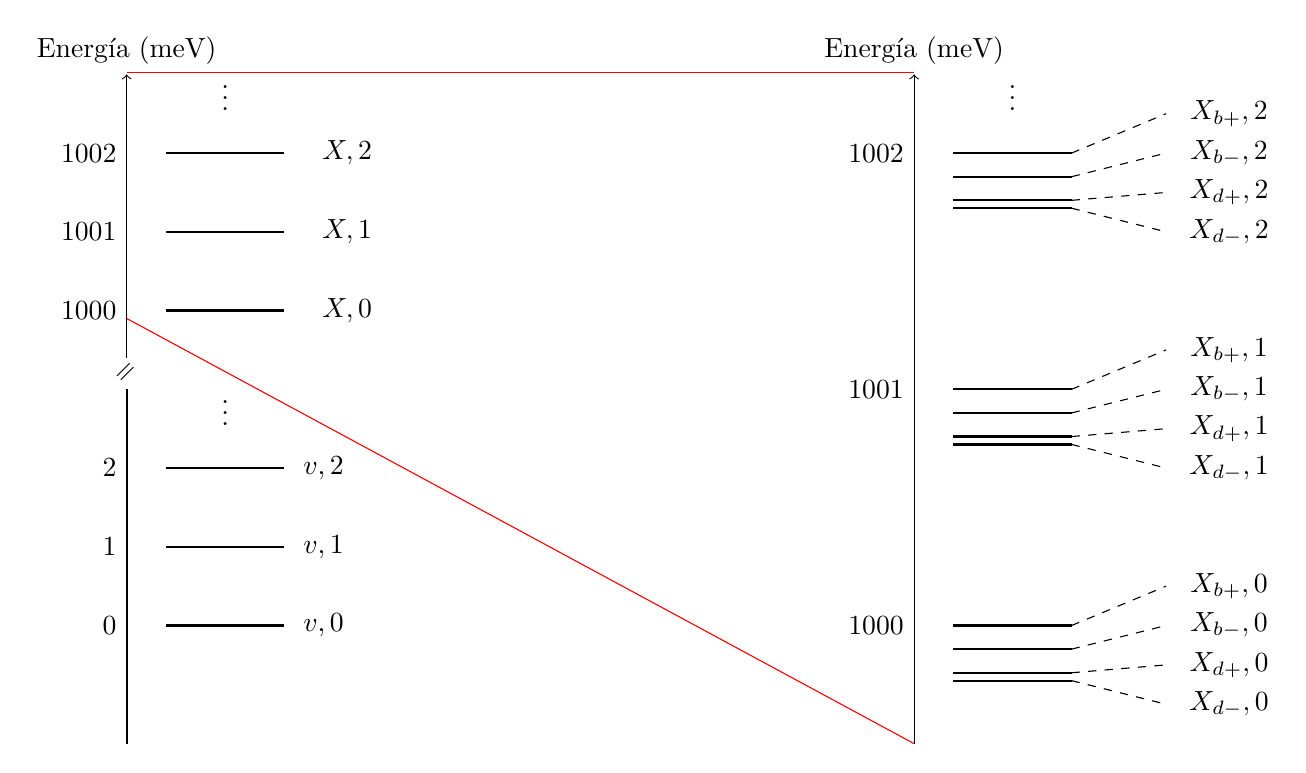
\begin{tikzpicture}[scale=1]
		% Ejes
		\draw[thick] (0,-1.5) -- (0,3);
		% quiebre del eje
		\node at (0,3.2) {\rotatebox{45}{$=$}};
		\draw[->] (0,3.4) -- (0,7) node[above] {Energía (meV)};
		
		% Niveles de energía
		\draw[thick] (0.5,0) -- (2,0) node[left] at (0,0) {0};
		\draw[thick] (0.5,1) -- (2,1) node[left] at (0,1) {1};
		\draw[thick] (0.5,2) -- (2,2) node[left] at (0,2) {2};
		%quiebre del eje
		\draw[thick] (0.5,4) -- (2,4) node[left] at (0,4) {1000};
		\draw[thick] (0.5,5) -- (2,5) node[left] at (0,5) {1001};
		\draw[thick] (0.5,6) -- (2,6) node[left] at (0,6) {1002};
		
		% Puntos suspensivos
		\node at (1.25,2.8) {\vdots};
		%quiebre del eje
		\node at (1.25,6.8) {\vdots};
		
		% Etiquetas de niveles
		\node at (2.5,0) {$\ket{v,0}$};
		\node at (2.5,1) {$\ket{v,1}$};
		\node at (2.5,2) {$\ket{v,2}$};
		%quiebre del eje
		\node at (2.8,4) {$\ket{X,0}$};
		\node at (2.8,5) {$\ket{X,1}$};
		\node at (2.8,6) {$\ket{X,2}$};
		
		\draw[red] (0,7.02) -- (10,7.02);
		\draw[red] (0,3.9) -- (10,-1.5);
		\begin{scope}[shift={(10,0)}]
			% Ejes
			\draw[->] (0,-1.5) -- (0,7) node[above] {Energía (meV)};
			
			% Niveles de energía
			\draw[thick] (0.5,-0.7) -- (2,-0.7);
			\draw[thick] (0.5,-0.6) -- (2,-0.6);
			\draw[thick] (0.5,-0.3) -- (2,-0.3);
			\draw[thick] (0.5,0) -- (2,0) node[left] at (0,0) {1000};
			
			\draw[thick] (0.5,2.3) -- (2,2.3);
			\draw[thick] (0.5,2.4) -- (2,2.4);
			\draw[thick] (0.5,2.7) -- (2,2.7);
			\draw[thick] (0.5,3) -- (2,3) node[left] at (0,3) {1001};
			
			\draw[thick] (0.5,5.3) -- (2,5.3);
			\draw[thick] (0.5,5.4) -- (2,5.4);
			\draw[thick] (0.5,5.7) -- (2,5.7);
			\draw[thick] (0.5,6) -- (2,6) node[left] at (0,6) {1002};
			
			% Puntos suspensivos
			\node at (1.25,6.8) {\vdots};
			
			% Etiquetas de niveles
			\draw[dashed] (2,-0.7) -- (3.2,-1) node at (4,-1) {$\ket{X_{d-},0}$};
			\draw[dashed] (2,-0.6) -- (3.2,-0.5) node at (4,-0.5) {$\ket{X_{d+},0}$};
			\draw[dashed] (2,-0.3) -- (3.2,0) node at (4,0) {$\ket{X_{b-},0}$};
			\draw[dashed] (2,0) -- (3.2,0.5) node at (4,0.5) {$\ket{X_{b+},0}$};
			
			\draw[dashed] (2,2.3) -- (3.2,2) node at (4,2) {$\ket{X_{d-},1}$};
			\draw[dashed] (2,2.4) -- (3.2,2.5) node at (4,2.5) {$\ket{X_{d+},1}$};
			\draw[dashed] (2,2.7) -- (3.2,3) node at (4,3) {$\ket{X_{b-},1}$};
			\draw[dashed] (2,3) -- (3.2,3.5) node at (4,3.5) {$\ket{X_{b+},1}$};
			
			\draw[dashed] (2,5.3) -- (3.2,5) node at (4,5) {$\ket{X_{d-},2}$};
			\draw[dashed] (2,5.4) -- (3.2,5.5) node at (4,5.5) {$\ket{X_{d+},2}$};
			\draw[dashed] (2,5.7) -- (3.2,6) node at (4,6) {$\ket{X_{b-},2}$};
			\draw[dashed] (2,6) -- (3.2,6.5) node at (4,6.5) {$\ket{X_{b+},2}$};	
		\end{scope}
	\end{tikzpicture}
	\caption{Diagrama de energ\'ia sin l\'aser $(\omega_L=0\text{meV})$ y sin campo magn\'etico $(B=0\text{T})$, con energia de excitaci\'on t\'ipica de los QDs $(\omega_b=1\text{eV})$. A la izquierda el diagrama de energia completo y a la derecha un acercamiento a la parte superior del diagrama debido a la gran cercan\'ia entre estados.}
\end{figure}

Para que se genere una oscilación de Rabi o una oscilación gigante-Rabi\footnote{La diferencia entre estas dos es cuán grande es la diferencia entre las frecuencias de excitación de los dos estados.}, es esencial que el estado del sistema sea una superposición con igual peso de dos estados de la base. Cuando se logra esta condición, se produce una oscilación de Rabi o gigante-Rabi, dependiendo de la estructura de los estados implicados. Esto implica que se debe modificar la estructura de los estados del sistema de tal manera que dos de ellos tengan la misma energía. Esta condición es fundamental para que los estados tengan igual peso en la superposición.

El parámetro inicial que elegimos para lograr esta condición es la energía del láser\footnote{Usando las unidades de energía cuando $\hbar =1$.}, que está inmersa en la definición del desafinamiento (o "detuning" en inglés) del sistema, $\Delta=\omega_b-\omega_L$, donde $\omega_b$ es la energía de excitación del excitón brillante y $\omega_L$ es la energía de excitación del láser de bombeo. Ajustando finamente la energía del láser, se encuentra que para ciertos valores, debido a la modificación de la estructura de estados por el desafinamiento, dos estados diferentes alcanzan la misma energía.

En este punto, el estado del sistema se encuentra en una superposición de dos estados de la base con igual peso, es decir,
\begin{equation}
	\ket{\psi} = c_1\ket{v,0} + c_2\ket{X,n}
\end{equation}
con $|c_1|^2=|c_2|^2$.

\section{Sin campo magn\'etico $(B=0 \text{\normalfont T})$}

En este apartado, se desea mostrar algunos detalles sobre la generación de las gigantes-Rabi, tomando como referencia el trabajo realizado por los autores \textcite{Vargas2022}. Primero, se presenta el diagrama de energías, donde se evidencia en qué puntos hay interacción y en cuáles no. En este diagrama, un cruce indica que no hay interacción, mientras que un anticruce señala que sí la hay. Este anticruce también se conoce como desdoblamiento de Rabi. Por lo tanto, se mostrarán los respectivos diagramas de dispersión para evidenciar lo mencionado anteriormente.

\begin{figure}[htbp]
	\centering
	\begin{subfigure}[b]{0.49\textwidth}
		\centering
		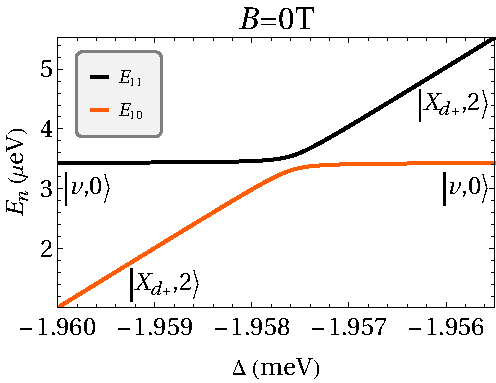
\includegraphics[width=\textwidth]{res/E11E10_B0}
		\caption{Anticruce, evidencia de interacción entre los estados propios de energía 10 y 11. En un valor de energ\'ia cerca a cero ($\sim$3.4 $\mu$eV).}
		\label{fig:E11E10_B0}
	\end{subfigure}
	\hfill
	\begin{subfigure}[b]{0.49\textwidth}
		\centering
		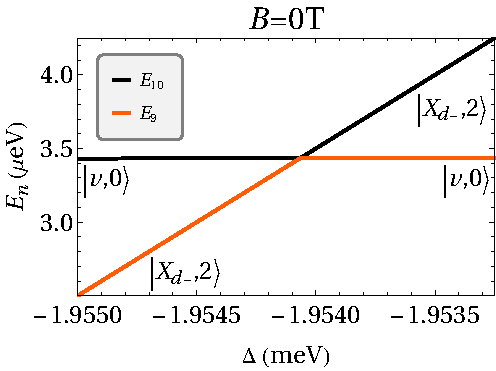
\includegraphics[width=\textwidth]{res/E10E9_B0}
		\caption{Cruce, muestra ausencia de interacción entre los estados propios de energía 9 y 10 con energ\'ia cerca a cero ($\sim$3.4 $\mu$eV).}
		\label{fig:E10E9_B0}
	\end{subfigure}
	\begin{subfigure}[b]{0.49\textwidth}
		\centering
		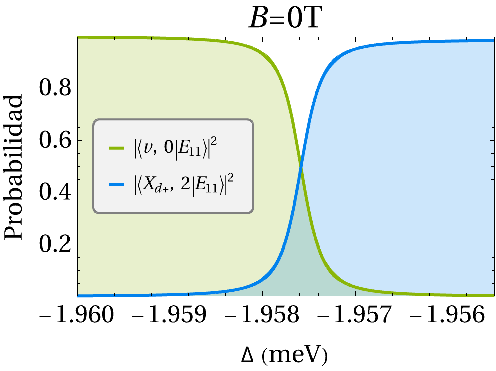
\includegraphics[width=\textwidth]{res/h11_B0}
		\caption{Coeficientes de Hopfield para observar cuáles son los estados de la base involucrados en la interacción.}
		\label{fig:sh11_B0}
	\end{subfigure}
	\hfill
	\begin{subfigure}[b]{0.49\textwidth}
		\centering
		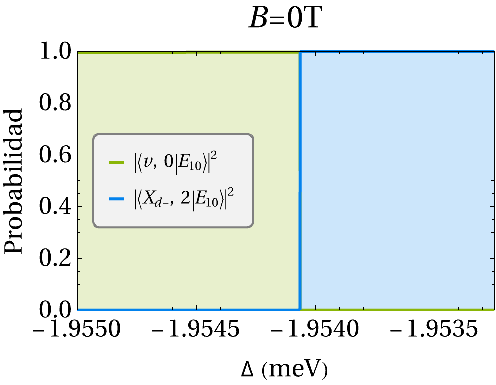
\includegraphics[width=\textwidth]{res/h10_B0}
		\caption{Coeficientes de Hopfield cuando se intercambian las etiquetas de los estados propios 9 y 10.}
		\label{fig:h10_B0}
	\end{subfigure}
	\begin{subfigure}[b]{0.49\textwidth}
		\centering
		\includegraphics[width=\textwidth]{res/ψ14_B0}
		\caption{Gigante-Rabi entre los estados de la base observados en los coeficientes de Hopfield.}
		\label{fig:ψ14_B0}
	\end{subfigure}
	\hfill
	\begin{subfigure}[b]{0.49\textwidth}
		\centering
		\includegraphics[width=\textwidth]{res/ψ15_B0}
		\caption{La ausencia de la gigante-Rabi, como se esperaba.}
		\label{fig:ψ15_B0}
	\end{subfigure}
	\caption{Aquí observamos dos procesos: a la izquierda, la obtención de la gigante-Rabi a partir del diagrama de dispersión, y a la derecha, cuando no se obtiene la gigante-Rabi.}
	\label{fig:Vladimir}
\end{figure}

El diagrama de energía se obtiene numéricamente, ordenando las energías de menor a mayor. De esta forma, también se organizan los vectores propios correspondientes. Esto implica que, cuando dos estados tienen la misma energía, el diagrama de dispersión mostrará un cruce y sus etiquetas se intercambiarán. Es decir, si el cruce ocurre entre los estados propios 9 y 10, después del cruce, el estado que era 9 pasará a ser 10 y viceversa, intercambiando así las etiquetas entre los estados propios.

Como se observa en la figura \ref{fig:Vladimir}, se detalla el procedimiento numérico para encontrar las gigantes-Rabi en general. Aquí se indica que cuando se encuentra un anticruce, se está evidenciando una interacción en la que, en principio, se intercambian los estados de la base entre los respectivos estados propios. Esto se puede comprobar usando los coeficientes de Hopfield, en los que se grafica la probabilidad de cada uno de los estados de la base de alguno de los dos vectores propios involucrados en la interacción.

Una vez se obtiene el valor del detuning, $\Delta \approx -n\omega_b$, cuyo valor es negativo debido a que el detuning se define como $\Delta = \omega_b - \omega_L$. Es decir, es negativo porque se está ajustando la energía del láser a un valor mayor que el de la excitación del excitón brillante, condición requerida para generar las gigante-Rabi entre un estado de menor variedad de excitación y uno de mayor variedad de excitación.

Si se quiere que el estado inicial del sistema sea el estado vacío $\ket{v,0}$, entonces se debe buscar el valor propio de energía más cercano a cero, además de considerar que la energía de estos estados también está cuantizada de acuerdo al número de fonones. Encontrar el valor de energía más cercano a cero en un detuning negativo indica que el sistema inicialmente se prepara en el estado vacío, para luego evolucionar a un estado excitón con $n$ fonones.

La variedad de excitación se entiende en este contexto como el número de excitación del modo fundamental del estado del sistema. El estado vacío tiene una variedad de excitación cero, mientras que el estado $\ket{n,X}$ tiene una variedad de excitación de $n+1$, donde $X$ indica cualquier estado excitón presente en el sistema, ya sean excitones brillantes u oscuros, que pueden ser simétricos o antisimétricos. Cuando la diferencia en la variedad de excitación es mayor a 1, se genera una gigante-Rabi.

\begin{figure}[hb]
	\centering
	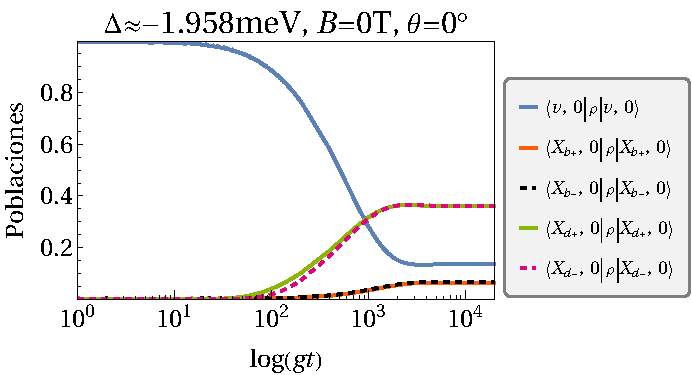
\includegraphics[width=0.7\linewidth]{res/ρ_B0}
	\caption{Din\'amica no unitaria del sistema usando los valores encontrados cuando el sistema esta cerrado.}
	\label{fig:b0}
\end{figure}

La gráfica muestra cómo la población del estado base disminuye a lo largo del tiempo mientras las poblaciones de los estados excitados aumentan, indicando una transferencia de población inducida por el bombeo del láser. El valor de \(\Delta\) juega un papel crucial en determinar qué estados excitados se pueblan más. Aquí, parece que el desafinamiento favorece la población de los estados \(\ket{X_{d+}}\) y \(\ket{X_{d-}}\).

\section{Configuraci\'on de Voigt $(\theta = 0^\circ)$}

\section{Configuraci\'on de Faraday $(\theta = 90^\circ)$}

\section{Descomposici\'on espectral}

A continuaci\'on se muestra el espectro de energ\'ias del sistema cuando no hay campo magn\'etico ($B=0$), es decir, el sistema modelado por \parencite{Vargas2022}. Se puede observar en la figura \ref{fig:energia-sin-campo-magnetico} que hay tres transiciones de estado permitidas y una prohibida a diferentes desafinamientos ($\Delta = \omega_b-\omega_L$) con $\omega_b$ siendo la energ\'ia de transici\'on del estado vac\'io ($\ket{v,0}$) al estado excit\'on brillante sim\'etrico ($\ket{X_{b+},0}$) y $\omega_L$ la energ\'ia del l\'aser. A continuaci\'on se muestran las transiciones permitidas con sus desafinamientos correspondientes y la transicion prohibida:
\begin{align}
	\bra{v,0}H\ket{X_{b+},2} &\neq 0 \quad \text{con} \quad \Delta \approx -2.001 \text{ meV},\\
	\bra{v,0}H\ket{X_{b-},2} &\neq 0 \quad \text{con} \quad \Delta \approx -1.981 \text{ meV},\\
	\bra{v,0}H\ket{X_{d+},2} &\neq 0 \quad \text{con} \quad \Delta \approx -1.957 \text{ meV},\\
	\bra{v,0}H\ket{X_{d-},2} &= 0 \quad \forall \;\; \Delta.
\end{align}



Como se puede observar la interacci\'on es del orden de los $\mu$eV obteniendo que la intensidad de la interaccion es la diferencia entre las energias correspondientes. As\'i si se activa el campo magneticos vamos a ver en la figura \ref{fig:detuning-con-campo-magnetico} si el minimo (donde sucede la interaccion entre estados) sufre algun cambio.

\begin{figure}[bh]
	\centering
	\includegraphics[width=.9\linewidth]{../res/det_θ0}
	\caption{Desfinamiento $\Delta$ variando la magnitud del campo magnetico horizontal $\theta=0$ rad, para la gigante-Rabi de cada estado exciton, son cuatro posibles permitidos con diferencia tres entre sus variedades de excitacion, donde se observa que $\Delta$ depende del campo magnetico al cadradado, $\Delta \sim B^2$, con algunas transiciones involucran dependencia lineal del campo magnetico.}
	\label{fig:det_θ0}
\end{figure}

En la figura \ref{fig:detuning-con-campo-magnetico} se observa que el desafinamiento depende de la intensidad campo magnetico horizontal y es diferente para cada una de las transiciones permitidas, ademas, habilita la transicion prohibida anteriormente sin campo magnetico. A continuacion menciono la funcion numerica relacionado con el corrimiento del desafinamiento que me permite producir oscilaciones gigante Rabi con diferencia 3 en las variedades de excitacion:
\begin{align}
	\bra{v,0}H\ket{X_{b+},2} &\quad \text{con} \quad \textcolor{magenta}{\Delta \approx -2.001\text{ meV} - 0.025B - 0.02B^2},\\
	\bra{v,0}H\ket{X_{b-},2} &\quad \text{con} \quad \textcolor{blue}{\Delta \approx -1.981\text{ meV} - 0.01B - 0.02B^2},\\
	\bra{v,0}H\ket{X_{d+},2} &\quad \text{con} \quad \textcolor{darkgreen}{\Delta \approx -1.957\text{ meV} - 0.02B^2},\\
	\bra{v,0}H\ket{X_{d-},2} &\quad \text{con} \quad \textcolor{red}{\Delta \approx -1.954\text{ meV} + 0.018B - 0.02B^2}.
\end{align}
%
\end{document}